
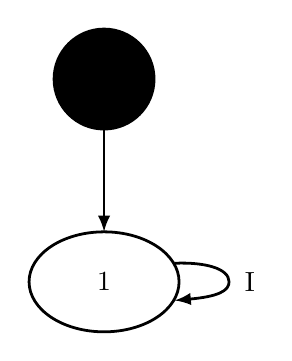
\begin{tikzpicture}[>=latex,line join=bevel,]
  \pgfsetlinewidth{1bp}
%%
\pgfsetcolor{black}
  % Edge: 0 -> 1
  \draw [->] (27bp,72.813bp) .. controls (27bp,64.789bp) and (27bp,55.047bp)  .. (27bp,36.029bp);
  % Edge: 1 -> 1
  \draw [->] (52.443bp,24.691bp) .. controls (63.028bp,25.152bp) and (72bp,22.922bp)  .. (72bp,18bp) .. controls (72bp,14.77bp) and (68.136bp,12.699bp)  .. (52.443bp,11.309bp);
  \definecolor{strokecol}{rgb}{0.0,0.0,0.0};
  \pgfsetstrokecolor{strokecol}
  \draw (79.5bp,18bp) node {I};
  % Node: 1
\begin{scope}
  \definecolor{strokecol}{rgb}{0.0,0.0,0.0};
  \pgfsetstrokecolor{strokecol}
  \draw (27bp,18bp) ellipse (27bp and 18bp);
  \draw (27bp,18bp) node {1};
\end{scope}
  % Node: 0
\begin{scope}
  \definecolor{strokecol}{rgb}{0.0,0.0,0.0};
  \pgfsetstrokecolor{strokecol}
  \definecolor{fillcol}{rgb}{0.0,0.0,0.0};
  \pgfsetfillcolor{fillcol}
  \filldraw [opacity=1] (27bp,91bp) ellipse (18bp and 18bp);
\end{scope}
%
\end{tikzpicture}

